%This is a very basic  BE PROJECT Synopsis template.


%############################################# 
%#########Author :  PROJECT Synopsis###########
%#########COMPUTER ENGINEERING############

%\title{SYNOPSIS}

\documentclass[16pt,oneside,a4paper]{article}

\usepackage{amsmath}
\usepackage{amssymb}
\usepackage{mathptmx}
\usepackage{amsfonts}
\usepackage{tikz}
\usetikzlibrary{shapes,arrows,positioning,fit}
\usepackage{color}
\usepackage{graphicx} % Required for the inclusion of images
\setlength\parindent{0pt} % Removes all indentation from paragraphs
\usepackage{times} 
\usepackage{fancyhdr}
\pagestyle{fancy}
\fancyhf{}
\fancyhead[C]{\LARGE SYNOPSIS}%Header of Document
\makeatletter
\let\ps@IEEEtitlepagestyle\ps@fancy
\makeatother

% Define block styles
\tikzstyle{decision} = [diamond, draw, fill=blue!20, 
    text width=4.5em, text badly centered, node distance=3cm, inner sep=0pt]
\tikzstyle{block} = [rectangle, draw, text width=5em, text centered, rounded corners, minimum height=4cm]
\tikzstyle{line} = [draw, -latex']
\tikzstyle{cloud} = [draw, circle, node distance=3cm,
    minimum height=2em]


%\usepackage{showframe}
%\hoffset = 8.9436619718309859154929577464789pt
%\voffset = 13.028169014084507042253521126761pt
\begin{document}
%\maketitle 
\section{Group Id}
Group ID.-3

\section{Project Title}
Voice Controlled Personal Assistant and Connecting IOT Devices
\section{ Project Option }
Internal Project

\section{Internal Guide}
Prof. Nitin R. Talhar


\section{Technical Keywords (As per ACM Keywords)}
 {\bfseries Technical Key Words:}      
 \begin{itemize}
 \item 	Special-Purpose and Application-Based System
 \item	Online Information Services
 \item  Natural Language Processing
 \item  Input/Output and Data Communication
 \item  Artificial Intelligence
 \item  Distributed System
 \item  Personal Computing
 \end{itemize}
%Please note ACM Keywords can be found : http://www.acm.org/about/class/ccs98-html \\
%Example is given as
%\begin{enumerate}
%	\item C. Computer Systems Organization 
%	\begin{enumerate}
%		\item C.2 COMPUTER-COMMUNICATION NETWORKS 
%		\begin{enumerate}
%			\item C.2.4 Distributed Systems 
%			\begin{enumerate}
%				\item  Client/server 
%\item Distributed applications
%\item Distributed databases
%\item Network operating systems 
%\item Distributed file systems
%\item Security and reliability issues in distributed applications
%	 		\end{enumerate} 
%		\end{enumerate} 
%	  
%
%	
%	\end{enumerate}
%\end{enumerate}



\section{Problem Statement}
\label{sec:problem}
To develop a hardware system which takes the input through voice commands and perform the various actions and keeps learning the context of these commands to further improvise the responses in future and help humans with day-to-day workforce.


\section{Abstract}
In the Modern Era of fast moving Technology we can do things which we never thought we could do before. But to achieve the accomplish these thought theres a need for a platform which can automate all our task with easy and comfort.\\

So there is a need to develop a voice controlled personal AI having brilliant powers of deduction and the ability to interact with our surroundings just by one of the materialistic form of human interaction, our VOICE. The Hardware device captures the personals audio request through microphone and  processes the request so that the device can respond to the individual using in-built speaker module.For Example, if you ask the device 'what's the weather?' or 'how's traffic?' using its built-in skills, it looks up the weather and returns the response to the customer through connected speaker.\\

\noindent
The platform is open to all and connect all IOT devices in the vicinity to perform the assigned task on go. This feature makes it distinctive from already existing personal AI’s and separates it from the flock. It uses open source software to process natural language, to determine the intent of the query and to perform the action. The platform features include : Turn on the lights, do the mathematics, play your favorite song or ask anything which comes to your mind. Just speak naturally and the platform is there to do your bidding.\\

\noindent
The Platform also a extends an Android Application in which you can add To-Do-list or set a reminder or alarm through the app, push notifications and personalize according to your needs. The device has a lot of native skills and abilities baked in it and more can be added to extend its capabilities.\\

\noindent
There is still a lot of ground to be covered up in the world of automation but the skills the device we are building posses, it can help to build a new generation of voice controlled devices and bring a new  sustaining change in the field of automation.\\

\section{Goals and Objectives}

\begin{itemize}
	\item The main objective of this device is to ease the burden of your work by providing any information you want and help you with daily work.
	\item To expedite you from the pressure of remembering things like meeting, play music on go, solve your queries.
	\item To develop a platform which can interact seamlessly and can have a friendly conversation with you.
	\item To control IOT devices of the surroundings of the device using simple commands.
\end{itemize}

	
\section{Relevant mathematics associated with the Project}
\label{sec:math}


System Description:
\begin{itemize} 
\item \textbf{Input:}	 
	\begin{itemize}
		\item Vocal Commands in Natural Language
		\item Creating and Updating To-Do List using Android Application
		\item Taking Picture using Android Application
	\end{itemize} 
\item \textbf{Output:}
	\begin{itemize}
		\item Vocal Reply of respective services to the query provided as Input.
		\item Reminder according to To-Do list.
		\item Picture Description of the Image Provided as Input.
	\end{itemize}	 
%\item Identify data structures, classes, divide and conquer strategies to exploit distributed/parallel/concurrent processing, constraints. 
%\item Functions : Identify Objects, Morphisms, Overloading in functions, Functional relations
\item \textbf{Mathematical Formulation:}\\
Let the M i the universal states which contains, \\
    \textbf{M = \{Q, S, F, Q1 , Qf \}} \newline
    where, \\
    \newline
    		Q = No. of states \{Q1,Q2,Q3,Q4,Q5,Q6,Q7,Q8\}\\
    		X = No. of states \{X1, X2, X3, X4\}\\
    		Q1 = Initial State.\\
    		S = Success state.\\
    		F = Failure state.\\
    		\newline
    where,\\ 
    \newline
    Q1= Start.\\
     \newline
    Q2 = Initialize assistant by calling "ARCKIN". \\
    \newline
    Q3 = Once initialized, give input in the speech format.\\
    \newline
    Q4 = Processing of speech into text.\\
    \newline 
    Q5 = Text is compared with commands.\\
    \newline
    Q6 = Perform action according to command.\\
    \newline 
    Q7 = Convert the action into speech.\\
    \newline 
    Q8 = Give output in the speech format.\\
    \newline
    X1 = Connect "ARCKIN" to mobile application.\\
    \newline
    X2 = Update To-Do list, Calender, Alarm, reminder, etc.\\
    \newline
    X3 = Updated data is sent to cloud server.\\
    \newline
    X4 = According to the data sent, "ARCKIN" will take action.\\
    \newline
    
\item \textbf{Failure Conditions:}  F = \{F1,F2,F3,S\} \newline
\begin{itemize}
\item F1  = Failure if the device is not initialised due to noisy background.
\item F2 = Connection with android app failed.
\item F3 = Server down failure or cannot retrieve data from server.
\end{itemize}

\item \textbf{Success Conditions:}
    \begin{itemize}
    		\item S1 = Success after the data is assimilated and output is produced accordingly.
	\end{itemize}     

\subsection{Activity Diagram}
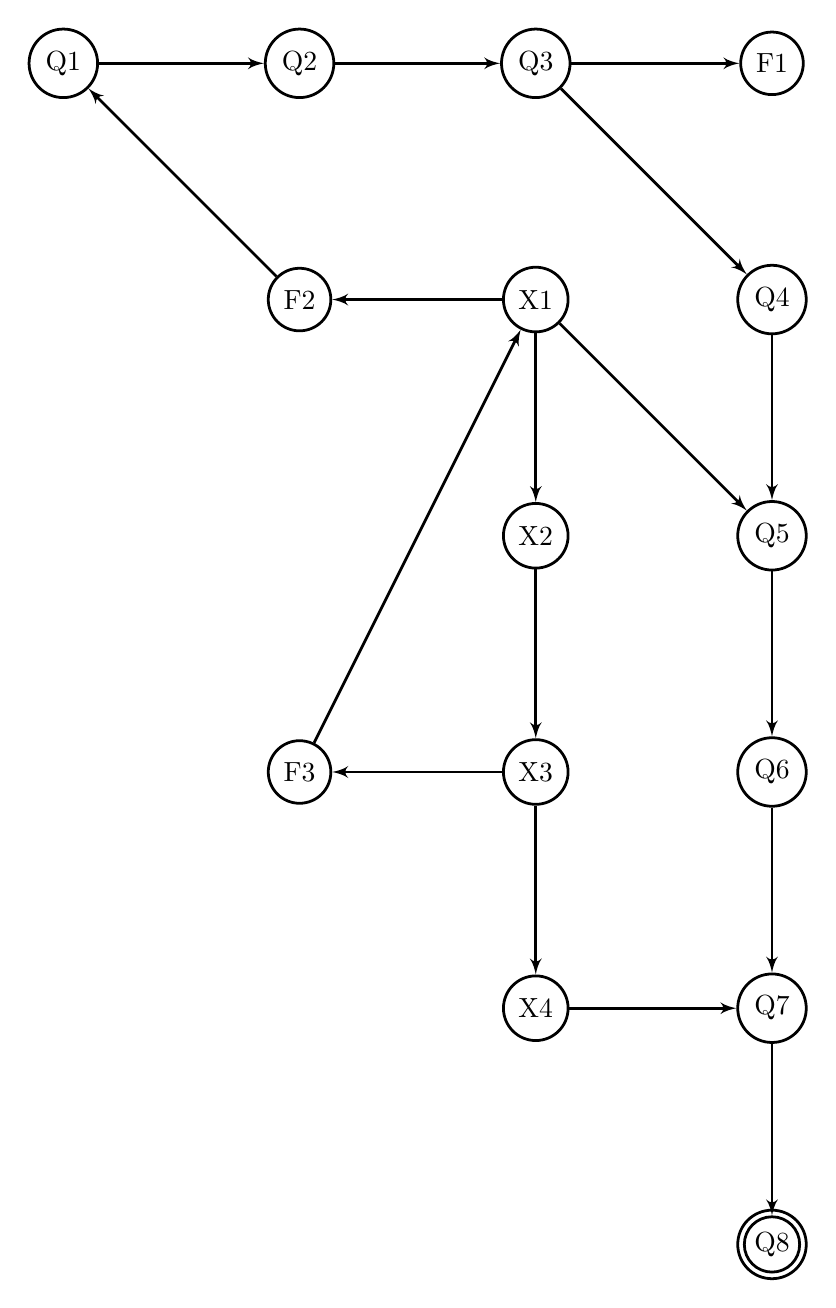
\begin{tikzpicture}[node distance = 6cm, auto, line width=1pt,>=latex]
    % Place nodes
    \node [cloud] (Q1) {Q1};
    \node [cloud, right of=Q1] (Q2) {Q2};
    \node [cloud, right of=Q2] (Q3) {Q3};
    \node [cloud, right of=Q3] (f1) {F1};
    \node [cloud, below of=f1] (Q4) {Q4};
    \node [cloud, below of=Q4] (Q5) {Q5};
    \node [cloud, below of=Q5] (Q6) {Q6};
    \node [cloud, below of=Q6] (Q7) {Q7};
    \node [cloud, below of=Q7] (Q8) {Q8};
    \node [cloud, left of=Q4] (x1) {X1};
    \node [cloud, left of=x1] (f2) {F2};
    \node [cloud, left of=Q5] (x2) {X2};
    \node [cloud, left of=Q6] (x3) {X3};
    \node [cloud, left of=x3] (f3) {F3};
    \node [cloud, left of=Q7] (x4) {X4};
    \node [cloud, below of=Q7] (Q8) {};
    % Draw edges
    \path [line] (Q1) -- (Q2);
    \path [line] (Q2) -- (Q3);
    \path [line] (Q3) -- (Q4);
    \path [line] (Q3) -- (f1);
    \path [line] (Q4) -- (Q5);
    \path [line] (x1) -- (f2);
    \path [line] (x3) -- (f3);
    \path [line] (Q5) -- (Q6);
    \path [line] (Q6) -- (Q7);
    \path [line] (Q7) -- (Q8);
    \path [line] (x1) -- (x2);
    \path [line] (x2) -- (x3);
    \path [line] (x3) -- (x4);
    \path [line] (x1) -- (Q5);
    \path [line] (x4) -- (Q7);
    \path [line] (f2) -- (Q1);
    \path [line] (f3) -- (x1);

    \end{tikzpicture}
	 		
\end{itemize}


\section{Names of Conferences / Journals where papers can be published}
\begin{itemize}
\item  International Conference on Human-Computer Interaction – INTERACT 2017 
\item  ICCE 2016 Sub-Conference on Artificial Intelligence in Education/Intelligent Tutoring Systems (AIED/ITS)
\item  ICHCIAI 2016 — International Conference Human Computer Interaction and Artificial Intelligence 
\item  Open Journal of Internet Of Things (OJIOT) 
\item  IEEE Intelligent Systems
\end{itemize}


\section{Review of Conference/Journal Papers supporting Project idea}
\label{sec:survey}
\begin{enumerate}
\item \textbf{Interacting With Computers by Voice: Automatic Speech Recognition and Synthesis -- \textit{DOUGLAS O’SHAUGHNESS}}\

This paper has examined the basic aspects of human–computer interactions via voice. The basic approaches and methods of ASR and synthesis have been discussed. Microprocessors can easily handle the computation speeds needed for many synthesizers, and many function entirely in software. However, the memory requirements of modern waveform concatenation systems strain the capacities of some practical systems.\\

\item \textbf{Analysis of Machine Translation and Speech Synthesis Speech-To-Speech Trnaslation System -- \textit{KEI HASHIMOTO, JUNICHI YAMAGISHI, WILLIAM BYRNE, SIMON KING, KEIICHI TOKUDA}}

This paper has provided an analysis of the impacts of machine translation and speech synthesis on speech-to-speech translation. We have shown that the naturalness and intelligibility of the synthesized speech are strongly affected by the fluency of the translated sentences. The intelligibility of synthesized speech is improved as the translated sentence become more fluent.\\

\item \textbf{On the track of Artificial Intelligence: Learning with Intelligent Personal Assistants -- \textit{NIL GOKSEL-CANBEK, MEHMET EMIN MUTLU}}

The paths of this study regarding IPAs is intended to reveal an overview on how and to what extent these devices might be used in human-computer interaction and learning. In this connection, the working systems of the IPAs namely Apple’s Siri, Google Now and Microsoft Cortana are revised within the context of AI. Although there have been several works related to IPAs in education. The potential use of IPAs for second language learning within Natural Language Processing (NLP) should be focused particularly.\\

\item \textbf{Chatbot-Assiting: SIRI -- \textit{HARSHITA PHATNANI, Mr. JYOTIPRAKASH PATRA, ANKIT SHARMA}}

Siri's first Apple iteration opens minds and speaks loudly to Siri's potential. What struck us is that even with this initial release one can readily imagine a sea change in the way humans interact with mobile. My voice application business allowed us to see the potential of truly great natural language voice technologies. The few great applications we found left us believing that someday, voice will handle large numbers of everyday tasks and, where appropriate, even more complex things.\\

\item \textbf{An Intelligent Voice Assistant Using Android Platform -- \textit{SUTAR SHEKHAR, POPHALI SAMEER, KAMAD NEHA, Prof. DEVKATE LAXMAN}}

We have developed application in which user can easily send a message with their voice commands and also tried to use the most of the inbuilt application with voice command. But all these applications have adaptions for the English language. We are also surveying to use the mailing and calendar where user will be able to mail and also create their event using voice command.\\

\item \textbf{Home Automation Using IOT  -- \textit{VINAY SAGAR, KUSUMA SM}}

Home automation using IOT has been experimentally proven to work satisfactorily by connecting simple appliances to it \& the application appliances were successfully controlled remotely through internet. The designed system not only monitors the sensor data like temperature, gas, light, motion sensors but also actuates a process according to the requirement. For instance, switching on the lights when it gets dark. It also stores the sensor parameters in the cloud in a timely manner. This will help user to analyze the condition of various parameters in the home anytime anywhere.\\

\item \textbf{RASPBERRY PI BASED ROBOT WITH CLOUD TECHNOLOGY -- \textit{ Prof. GOKILAVANI R, NAVANEETHAN S}}

The data monitored has been updated to the firebase cloud server with the help of wifi \& the continuous access from anywhere is feasible. The proposed method contains the raspberry pi and the sensor devices. The output sensor data is updated to the cloud server; the updated sensor values can be viewed on its own smart phone. The commands can be sent to server by using wifi using the IP address of raspberry pi toolkit. \\


\item \textbf{Exploring IOT Application Using Raspberry Pi -- \textit{CHEAH WAI ZHAO, JAYANAND JEGATHEESAN, SON CHEE LOON}}

Raspberry PI is useful for small application development because it can be used to integrate with many components such as speakers, LED lights, sensors, cameras and wireless communication units to develop smart applications. It is very important to protect the file in order to maintain data consistency and accuracy. File sharing is widely used ranging from small-medium sized company to big company. One of the reason is that, admin can easily manage the file and client can access the file efficiently.\\

\pagebreak

\item \textbf{Natural Language Processing -- \textit{ABHIMANYU CHOPRA, ABHINAV PRASHAR, CHANDRESH SAIN}}

The strength of the capabilities to use natural language for query specification and retrieval bags over the keyword, key-phrase approaches. We believe that the restricted use of natural language in captions for multimedia data abstraction is less cumbersome task than the full natural language fact abstraction and feel that can be judged and build upon not only for abstracting images but also the form so multimedia (audio, video, text, data etc) data as input sources.\\

\item \textbf{A study of techniques for facial detetection and expression classification -- \textit{G. HEMALATHA, C.P. SUMATHI}}

Although human recognize facial expressions virtually without effort or delay, reliable expression recognition by machine is still a challenge, in achieving aptimal preprocessing, feature extraction or selection, and classificaton, particularly under conditions of input data variability.To attain successful recognition performance, most current expression recognition approaches require some control over the imaging conditions because many rea;-world applications requires operational flexibility.\\

\end{enumerate}

\section{Plan of Project Execution}
\begin{center}
	\begin{figure}[h]
	\centering 
	\includegraphics[scale=0.7]{gant2.jpg}
	\end{figure}
	
	\includegraphics[scale=0.65]{gant1.jpg}
\end{center}


\end{document}